Usual SC with a brief exploration of thin film SC.

\begin{parts}
	\part From the BCS theory, we know that due to the attractive phonon interaction, electrons pair up to form Cooper pairs via the Pauli exclusion principle.
	
	Since this interaction is attractive, there is 
	an energy saving by the electrons at Fermi surface to form Cooper pairs, and this leads to the opening of an energy gap as those electrons are now in the SC phase and form a condensate.
	
	\begin{figure}[H]
		\centering
		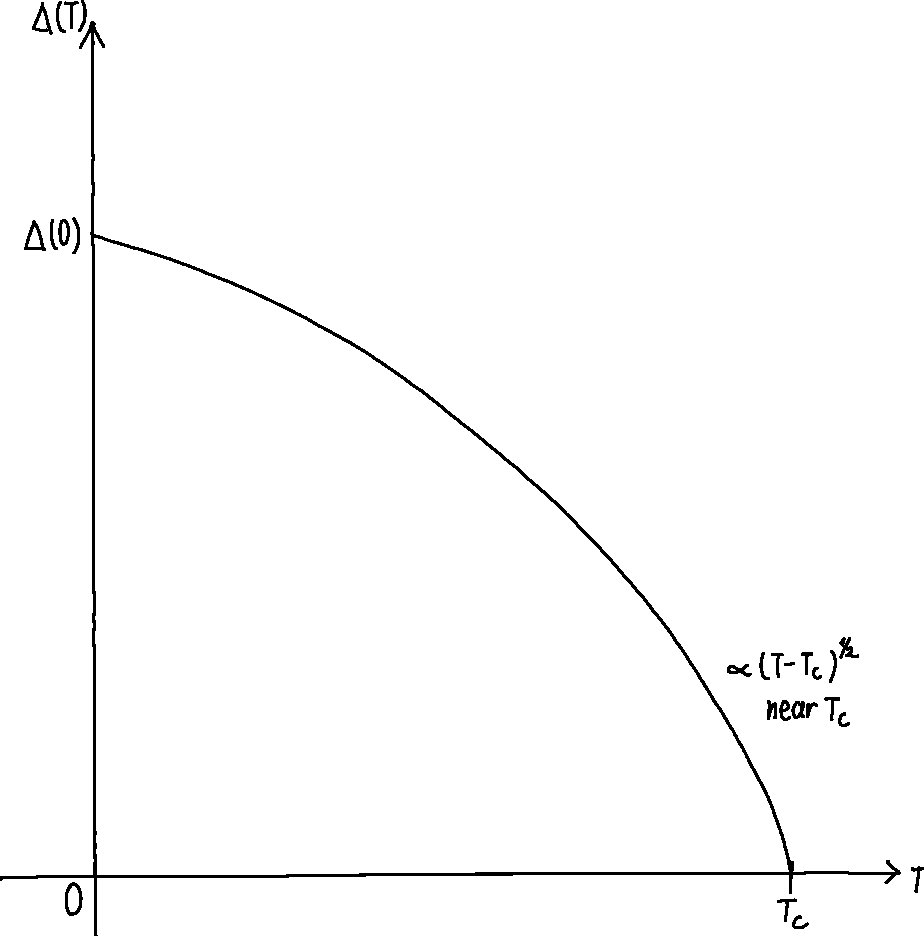
\includegraphics[width=.8\linewidth]{q3-energy-gap}
	\end{figure}
	
	Since $\Delta$ relates to the SC carrier density $n_s$, it follows that near $T_c$ it exhibits the same $T$ dependence as $\psi = \sqrt{n_s} \mathrm{e}^{i\theta}$.
	
	To explore the momentum dependence of $\Delta$, we may perform a measurement of tunnelling current through the SC.
	The bias voltage simply adjusts the explored energy level.
	
	\newpage
	
	\part Sketch of the setup:
	\begin{figure}[H]
		\centering
		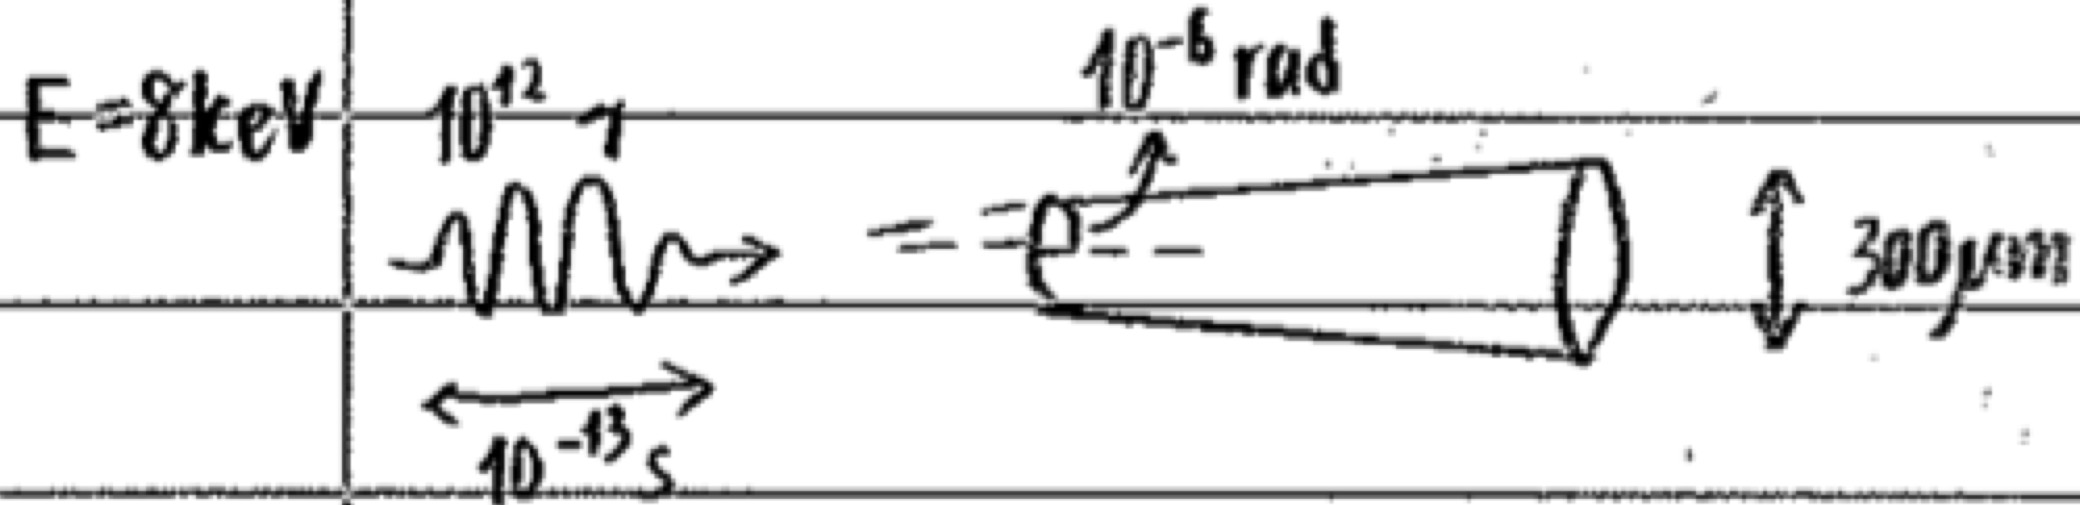
\includegraphics[width=.6\linewidth]{q3-setup}
	\end{figure}
	
	From Maxwell,
	\begin{align*}
		\mathbf{\nabla} \times \mathbf{B} &= \mu_0 \mathbf{J} \\
		\begin{vmatrix}
			\hat{\mathbf{x}} & \hat{\mathbf{y}} & \hat{\mathbf{z}} \\
			\partial_x & \partial_y & \partial_z \\
			0 & 0 & B
		\end{vmatrix} &= \mu_0 \mathbf{J} \\
		\Rightarrow \mu_0 \mathbf{J} &= -\pdiff{x}\rbracket{B_0 \frac{\cosh\rbracket{x/\lambda}}{\cosh\rbracket{t/\lambda}}} \hat{\mathbf{y}} \\
		\mathbf{J} &= -\frac{B_0}{\mu_0 \lambda} \frac{\sinh\rbracket{x/\lambda}}{\cosh\rbracket{t/\lambda}} \hat{\mathbf{y}}
	\end{align*}
	
	\newpage
	
	Sketch of $J$ along $x$:
	\begin{figure}[H]
		\centering
		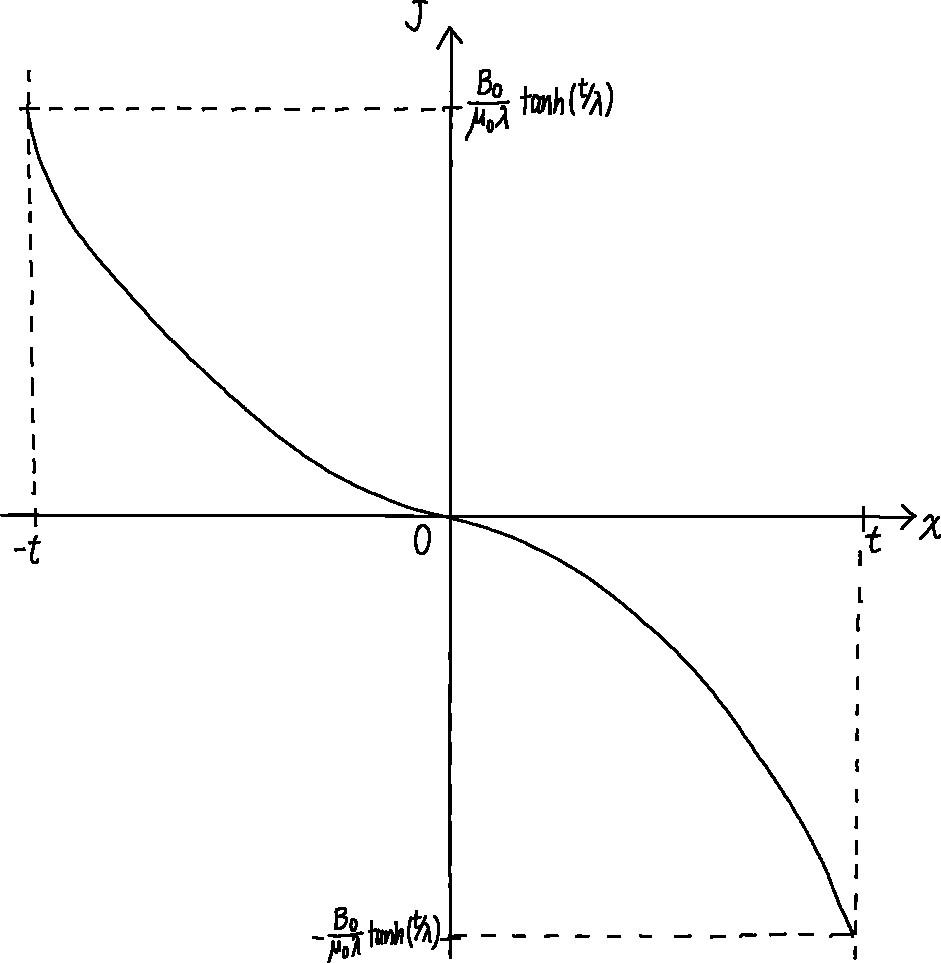
\includegraphics[width=.8\linewidth]{q3-j}
	\end{figure}
	
	For $\lambda \gg t$, we see that $B(x) \rightarrow B_0 \sbracket{1 + \mathcal{O}\rbracket{x^2/\lambda^2}}$ so we have the B field virtually penetrating the sample.
	
	Critical current density wise, it follows from the graph that it must also shrink to 0.
	
	\part $\kappa = \lambda/\xi = 100 > 1/\sqrt{2}$ $\Rightarrow$ type-II so vortex formation favourable.
	
	Extrapolating from the graph gives us $B_{c2} \simeq \SI{100}{\tesla}$.
	
	Also for type-II SC, upper field corresponds to when $\rbracket{2\pi\xi^2}B_c \Phi_0$ where $\xi$ is coherence length:
	\begin{gather*}
		\rbracket{2\pi\xi^2}B_c \Phi_0 = \SI{100}{\tesla} \\
		\Rightarrow \xi = \SI{1.81}{\nano\metre}
	\end{gather*}
	Hence:
	\begin{equation*}
		\lambda = \xi\kappa = \SI{181}{\nano\metre}
	\end{equation*}
	
	Now we have:
	\begin{align*}
		\xi &= \frac{\hbar v_\textnormal{F}}{\pi\Delta} \\
		\Rightarrow \Delta &= \frac{\hbar v_\textnormal{F}}{\pi\xi} = \SI{0.18}{\electronvolt}
	\end{align*}
	
	From BCS theory we have $\Delta(0) = 2\hbar\omega_D \mathrm{e}^{-1/\lambda}$ and $k_\textnormal{B}T_\textnormal{c} = 1.13\hbar\omega_D \mathrm{e}^{-1/\lambda}$:
	\begin{align*}
		\Rightarrow \Delta(0) &\simeq 1.77k_\textnormal{B} T_\textnormal{c} \\
		&\simeq \SI{5.34e-3}{\electronvolt} \textnormal{\hspace{1em}for $T_\textnormal{c} \simeq \SI{35}{\kelvin}$}
	\end{align*}
	Since there is a huge difference between the 2 predictions, this SC may not be explained by BCS theory (unless strong phonon interaction is accounted for).
\end{parts}